% IE Research Capstone Thesis -- compliant with Kick-Off May 2026 guidelines:
% max 30 pages (excl. refs/appendices), 12pt Times New Roman, 1.5 line spacing,
% structure: Cover / Abstract / Intro / Lit Review / Methodology / Results /
% Discussion / Conclusions / References (IEEE) / Appendices (Annex A: ICS).
\documentclass[12pt]{article}

\usepackage[utf8]{inputenc}
\usepackage[T1]{fontenc}
\usepackage{amsmath,amssymb}
\usepackage{amsthm}                      % before newtxmath to avoid \openbox clash
\let\openbox\relax
\usepackage{newtxtext,newtxmath}        % Times New Roman text + math
\usepackage[margin=1in]{geometry}
\usepackage{setspace}\onehalfspacing    % 1.5 line spacing
\usepackage{booktabs,array,enumitem,graphicx,xcolor,mathtools}
\usepackage{algorithm}
\usepackage[noend]{algpseudocode}
\usepackage[hidelinks]{hyperref}
\usepackage[numbers,sort&compress]{natbib}  % IEEE-style numeric citations

\newtheorem{proposition}{Proposition}
\newcommand{\vecx}{\operatorname{vec}}
\newcommand{\Cov}{\operatorname{Cov}}
\newcommand{\CVaR}{\mathrm{CVaR}}
\newcommand{\R}{\mathbb{R}}
\newcommand{\E}{\mathbb{E}}
\newcommand{\chiU}{\chi_{\mathrm{U}}}
\newcommand{\chiL}{\chi_{\mathrm{L}}}
\newcommand{\gco}{\mathrm{gCO_2eq/kWh}}

\begin{document}

% ===================== COVER PAGE =====================
\begin{titlepage}
\centering
{\large IE University --- School of Science \& Technology\par}
\vspace{0.4cm}
{\large Master in Business Analytics \& Data Science\par}
{\large Research Capstone in Operations Research\par}
\vspace{2.2cm}
{\Large\bfseries Does Spatial Correlation of Carbon Intensity Improve\par
Distributionally Robust Carbon-Aware Data-Center Scheduling?\par}
\vspace{0.5cm}
{\large A Multi-Grid Falsification Study with a Causal Mechanism\par}
\vspace{2.2cm}
{\large\bfseries Marco Ortiz Togashi\par}
\vspace{0.3cm}
{\large Supervisor: Prof.\ Bissan Ghaddar\par}
\vspace{2.2cm}
{\large June 2026\par}
\vfill
\begin{minipage}{0.9\textwidth}\small
\textbf{AI Use Declaration.} Generative AI tools (Anthropic Claude) were used as a
research and engineering assistant under the author's direction: for code
implementation support, experiment orchestration, literature triage, and drafting
assistance. All research questions, modelling decisions, experimental designs, and
interpretations are the author's, developed with the supervisor; all results were
produced by version-controlled, pre-registered code reviewed by the author, and all
text was reviewed and edited by the author.
\end{minipage}
\end{titlepage}

% ===================== ABSTRACT =====================
\begin{abstract}
\noindent Carbon-aware schedulers shift data-center compute toward hours and regions
where electricity is cleanest, and recent work models carbon intensity as uncertain
within a distributionally robust optimization (DRO) framework. A natural next step
is to treat carbon intensity as a stochastic \emph{vector} across electrically
coupled regions, so that \emph{spatial correlation} can inform the schedule. This
thesis asks whether that spatial structure carries any robust scheduling value.
Using a Mahalanobis--Wasserstein DRO formulation solved as a second-order cone
program, we design a falsification test --- the schedule fitted to the joint
covariance versus one fitted to a block-diagonal covariance with all cross-region
structure destroyed --- evaluated by out-of-sample $\CVaR_{0.95}$ of daily emissions
under strict pre-registration. Across three primary US/Canada grids spanning the
dependence spectrum --- the US West (California, Nevada, Phoenix), an
Ontario-anchored Eastern Interconnection belt, and an engineered heterogeneous
solar/wind/hydro portfolio --- corroborated by an Iberia--France panel as a
low-correlation anchor, the answer is a replicated, robustness-checked \textbf{null}: the spatial gap never
exceeds a few tenths of one percent, survives shrinkage and residualization
batteries, Benjamini--Hochberg correction, and walk-forward validation. Two
diagnostics explain the mechanism. A \emph{mean-ablation} experiment shows the
covariance signal is genuine and exploitable but dominated by the mean carbon
field; a \emph{tail-dependence} analysis shows the residual dependence is
non-elliptical --- upper-tail-independent and radially asymmetric --- and thus
structurally invisible to covariance-based ambiguity sets. A second phase
forecloses the obvious objection by replacing the covariance ball with Gaussian and
lower-tail (Clayton) copula schedulers that \emph{can} represent the asymmetry: the
null survives intact, and a mean-dominance bound grounded in the translation
invariance of CVaR explains why no passive dependence model can help. The practical
recommendation is that per-region marginal schedulers capture essentially all the
value; spatial value, if any, must come from an active transfer channel rather than
a richer dependence model.
\end{abstract}
\newpage
\tableofcontents
\newpage

% ===================== 1. INTRODUCTION =====================
\section{Introduction}\label{sec:intro}

\subsection{Context}
Data centers consumed an estimated 1--2\% of global electricity and their demand is
growing rapidly with AI workloads \citep{iea2024}. Unlike most industrial loads,
compute is unusually \emph{flexible}: many batch and training workloads can be
delayed by hours or moved between sites with little loss of utility. Because the
carbon intensity of grid electricity varies strongly by hour and by region ---
driven by wind, solar, hydro availability, and demand --- this flexibility lets a
data-center operator act as a grid-aware participant, deferring work from dirty
hours to clean ones \citep{radovanovic2022,wiesner2021}. Google's carbon-intelligent
computing platform demonstrated such temporal shifting at production scale
\citep{radovanovic2022}, and recent systems work extends it to variable-capacity
operation \citep{wijayawardana2025}.

Scheduling against \emph{tomorrow's} carbon intensity, however, means scheduling
under uncertainty. Distributionally robust optimization (DRO) addresses this by
optimizing against the worst distribution in an ambiguity ball around the empirical
distribution \citep{esfahani2018}, and has been applied to carbon-aware scheduling
with carbon intensity as the uncertain quantity \citep{hall2024}. Existing
formulations treat each region's carbon intensity essentially in isolation. Yet
carbon intensities of electrically interconnected regions co-move: weather fronts
traverse neighbouring balancing areas, and shared solar fleets create synchronized
clean periods. It is therefore natural to model carbon intensity as a stochastic
\emph{vector} with a full spatial covariance --- the extension studied here.

\subsection{Problem statement and research questions}
Modelling spatial dependence is not free: cross-region covariance blocks must be
estimated from limited data, and a richer uncertainty model is only worthwhile if it
buys measurably better schedules. The literature has assumed, rather than tested,
that spatial correlation in the carbon field is worth modelling. This thesis tests
that assumption directly.

\begin{description}[leftmargin=1.4em,itemsep=2pt]
\item[RQ1.] Is the carbon intensity of electrically coupled regions genuinely
spatially correlated, beyond shared diurnal cycles?
\item[RQ2.] Does feeding that spatial correlation to a covariance-based
(Mahalanobis--Wasserstein) DRO scheduler reduce out-of-sample tail emissions
($\CVaR_{0.95}$), relative to an otherwise identical scheduler that ignores
cross-region dependence?
\item[RQ3.] If not, \emph{why} not --- and what dependence structure, if any,
would a richer uncertainty model need to capture?
\end{description}

\subsection{Contributions}
The thesis makes four contributions. (i)~\emph{A falsification design}: a
shuffled-marginals test that isolates exactly the value of spatial covariance,
evaluated out-of-sample under pre-registration discipline (commit-locked
configurations, dry-run gates, single test-set read). (ii)~\emph{A replicated
empirical null across the dependence spectrum}: three primary US/Canada region sets
--- two interconnected grids where strong correlation survives de-seasonalization
(the US West --- California, Nevada, Phoenix; and an Ontario--Eastern belt) and one
engineered near-uncorrelated solar/wind/hydro portfolio --- corroborated by an
Iberia--France panel where residual correlation collapses to the diurnal cycle, all
yielding spatial gaps below $0.4\%$ of $\CVaR$,
robust to estimator choice, multiple-testing correction, and walk-forward
validation. (iii)~\emph{A causal mechanism}: a mean-ablation experiment showing the
covariance signal is real but dominated by the mean field, and a tail-dependence
analysis showing the residual dependence is non-elliptical
(upper-tail-independent, radially asymmetric), hence invisible to covariance-based
ambiguity sets by construction. (iv)~\emph{Practice and theory implications}: a
per-region marginal scheduler captures essentially all attainable value, and the
evidence yields a precise specification mandate for copula-based DRO.

\subsection{Thesis structure}
Section~\ref{sec:lit} reviews the literature and locates the gap.
Section~\ref{sec:method} develops the optimization model, the falsification test,
and the evaluation protocol. Section~\ref{sec:results} reports the correlation
validation and the experimental results across all region sets, including the
robustness battery, mean-ablation, tail-dependence diagnostics, and the Phase 2
copula schedulers.
Section~\ref{sec:discussion} interprets the findings against prior work and states
limitations. Section~\ref{sec:conclusion} concludes and outlines future work.

% ===================== 2. LITERATURE REVIEW =====================
\section{Literature Review}\label{sec:lit}

\subsection{Carbon-aware computing}
Carbon-aware scheduling exploits temporal and spatial variation in grid carbon
intensity. In production at Google, Radovanovi\'c et
al.~\citep{radovanovic2022} describe a system which
computes day-ahead ``virtual capacity curves'' that throttle flexible compute during
high-carbon hours; measured impact on latency-sensitive workloads is negligible
while load shifts measurably toward cleaner hours. Wiesner et al.~\citep{wiesner2021} analyse the
potential of temporal shifting across regions and workloads, finding the benefit
depends strongly on the grid's marginal mix and the workload's flexibility.
Wijayawardana and Chien~\citep{wijayawardana2025} study cloud-VM scheduling on datacenters whose capacity
varies with grid conditions --- including carbon-coupled capacity, where a constant
carbon budget forces capacity to fall as intensity rises --- and document the
goodput cost of capacity variation for long-running jobs. This systems literature
establishes operational levers (deferral, throttling, capacity coupling) that we
adopt as constraints, but it treats future carbon intensity as a point forecast;
uncertainty is handled implicitly, by re-planning.

\subsection{Distributionally robust optimization}
DRO optimizes against the worst-case distribution within an ambiguity set, and the
Wasserstein ball around the empirical distribution has emerged as the canonical
data-driven choice, with tractable finite-dimensional reformulations
\citep{esfahani2018,kuhn2019}. For costs linear in the uncertain vector, type-2
Wasserstein DRO with a Mahalanobis ground metric reduces to a mean term plus a
covariance-weighted regularizer --- an interpretable ``mean plus
$\varepsilon\,\sqrt{x^\top\Sigma x}$'' objective solvable as a second-order cone
program (SOCP) \citep{blanchet2019}. Hall et al.~\citep{hall2024} apply Wasserstein DRO to
carbon-aware data-center scheduling with virtual capacity curves, treating each
region's carbon intensity as the uncertain quantity and demonstrating robustness
gains over sample-average approximation. The risk functional we target,
$\CVaR_{\beta}$, is standard for tail-focused evaluation \citep{rockafellar2000}.
Beyond second moments, recent work robustifies the \emph{dependence structure}
itself: Fan et al.~\citep{fan2024} place both the marginals and the \emph{copula} within a
Wasserstein ball, the natural home for the non-elliptical structure our Phase 2
copula schedulers target.

\subsection{Spatial dependence and its modelling}
Cross-region dependence enters a Mahalanobis--Wasserstein model only through the
off-diagonal blocks of the covariance matrix. Estimating large covariance matrices
from short panels is noisy; shrinkage estimators \citep{ledoit2004} are the standard
remedy and serve here as a robustness arm. Beyond second moments, dependence is
fully described by the copula \citep{sklar1959,joe2014}; tail-dependence
coefficients quantify joint extremes that correlation cannot see, and the Gaussian
copula has zero asymptotic tail dependence for any correlation below one
\citep{embrechts2002} --- a property we exploit as a diagnostic benchmark.
Vine-copula constructions make high-dimensional non-elliptical dependence tractable
\citep{joe2014} and are the natural candidate for a dependence-aware extension of
DRO ambiguity sets.

\subsection{The gap}
To our knowledge, no prior work \emph{tests} whether spatial correlation of carbon
intensity --- however strong in the data --- translates into out-of-sample robust
scheduling value. The systems literature does not model uncertainty explicitly; the
DRO literature models uncertainty per region but has not isolated the marginal
contribution of \emph{cross-region} dependence; and neither offers a controlled
mechanism for \emph{why} spatial structure should or should not matter. This thesis
fills that gap with a falsification test, a replicated multi-grid study, and two
mechanism diagnostics (mean-ablation and tail dependence).

% ===================== 3. METHODOLOGY =====================
\section{Methodology}\label{sec:method}

\subsection{Research design overview}
The design is a controlled computational experiment. We hold the optimization
machinery fixed and manipulate exactly one object --- the cross-region blocks of the
covariance supplied to the scheduler --- then measure the consequence on held-out
tail emissions. Three primary region sets spanning the dependence spectrum (with two
earlier panels corroborating) serve as replications; three nested constraint regimes
guard against the result being an
artifact of a particular feasible-set geometry; a robustness battery (estimators,
multiple-testing correction, walk-forward) guards against statistical artifacts; and
two further experiments (mean-ablation; tail dependence) identify the mechanism.
Throughout, a pre-registration discipline removes analyst degrees of freedom.

\subsection{The scheduling problem}
Compute is scheduled across $R$ regions over a $T=24$-hour day. The decision is
$x\in\R^{R\times T}_{\ge0}$, where $x_{r,t}$ is compute power (MW) in region $r$ at
hour $t$. Carbon intensity $\rho_{r,t}$ ($\gco$) is uncertain; realized emissions
are linear, $\langle\rho,x\rangle=\sum_{r,t}\rho_{r,t}x_{r,t}$.

\subsection{Distributionally robust formulation}
We minimize worst-case expected emissions over a type-2 Wasserstein ball
$\mathcal{B}_\varepsilon(\hat{\mathbb{P}})$ of radius $\varepsilon$ centred on the
empirical distribution of the daily carbon field, with Mahalanobis ground metric
induced by the empirical covariance $\hat\Sigma\in\R^{RT\times RT}$:
\begin{equation}
\min_{x\in\mathcal{X}}\ \sup_{\mathbb{Q}\in\mathcal{B}_\varepsilon(\hat{\mathbb{P}})}
\E_{\mathbb{Q}}\big[\langle\rho,x\rangle\big]
\;=\;
\min_{x\in\mathcal{X}}\ \langle\bar\rho,x\rangle
+\varepsilon\sqrt{x^\top\hat\Sigma\,x},
\label{eq:obj}
\end{equation}
by Wasserstein duality for linear costs \citep{esfahani2018,blanchet2019}, where
$\bar\rho$ is the empirical mean field. With the Cholesky factorization
$\hat\Sigma=LL^\top$ the penalty becomes $\varepsilon\lVert
L^\top\vecx(x)\rVert_2$. Introducing an epigraph variable $t$, \eqref{eq:obj} is the
second-order cone program
\begin{equation}
\min_{x\in\mathcal X,\,t\ge0}\ \langle\bar\rho,x\rangle+\varepsilon\,t
\quad\text{s.t.}\quad \big\lVert L^\top\vecx(x)\big\rVert_2\le t,
\label{eq:socp}
\end{equation}
solved to global optimality (CLARABEL). The radius $\varepsilon$ interpolates from
the deterministic LP ($\varepsilon=0$) to increasingly conservative schedules.

\paragraph{Where spatial correlation enters.}
Partitioning $\hat\Sigma$ into $T\times T$ blocks $\Sigma_{rs}$ by region pair, the
quadratic form splits as
\begin{equation}
x^\top\hat\Sigma x=\sum_r x_r^\top\Sigma_{rr}x_r
+\sum_{r\neq s}x_r^\top\Sigma_{rs}x_s ,
\label{eq:quad}
\end{equation}
so the off-diagonal (spatial) blocks are the \emph{only} channel by which
cross-region dependence can alter the schedule. The experiment manipulates exactly
these blocks.

\subsection{Feasible set and constraint regimes}\label{sec:constraints}
The feasible set $\mathcal{X}$ collects the linear constraints below; introducing an
auxiliary flexible-load variable $x^{\mathrm f}\in\R^{R\times T}_{\ge0}$, the
scheduler solves \eqref{eq:obj} over
\begin{subequations}\label{eq:feasible}
\begin{align}
&0\le x_{r,t}\le\bar x_{r,t}, && \forall r,t
  &&\text{(C0: capacity)}\\[2pt]
&x_{r,t}=\alpha_r W_r\,p_{r,t}+x^{\mathrm f}_{r,t}, && \forall r,t
  &&\text{(C2: flex/inflex split)}\\[2pt]
&\textstyle\sum_{t} x^{\mathrm f}_{r,t}=(1-\alpha_r)\,W_r, && \forall r
  &&\text{(C2: work conservation)}\\[2pt]
&\lvert x_{r,t}-x_{r,t-1}\rvert\le\Delta_r, && \forall r,t
  &&\text{(C3: ramp)}\\[2pt]
&\textstyle\sum_{t\in\mathcal W} x^{\mathrm f}_{r,t}\ge\gamma\,(1-\alpha_r)\,W_r,
  && \forall r &&\text{(3a: deferral deadline)}\\[2pt]
&\pi_{r,t}\,x_{r,t}\le\bar P, && \forall r,t
  &&\text{(3b: thermal/PUE)}\\[2pt]
&\textstyle\sum_{r,t}\bar\rho_{r,t}\,x_{r,t}\le B
  && &&\text{(3d: carbon budget)}
\end{align}
\end{subequations}
where $W_r$ is region $r$'s daily work (utilization fixed at $80\%$, $W_r=960$ MWh);
$\alpha_r\in\{0.30,0.50,0.75\}$ is the inflexible fraction following the fixed
intraday shape $p_{r,t}$ ($\sum_t p_{r,t}=1$); $\Delta_r=15$ MW/h is the ramp limit;
$\mathcal W=[0,7]$ and $\gamma=0.20$ set the deferral deadline; and
$\pi_{r,t}=\mathrm{PUE}_0+\kappa\max(\mathcal T_{r,t}-\mathcal T_{\mathrm{set}},0)$
is the temperature-coupled power-usage multiplier (data, hence a constant per cell),
capped at effective power $\bar P$. Every constraint is linear, so $\mathcal X$ is
polyhedral and the program \eqref{eq:obj} remains an SOCP.

The capacity ceiling is constant ($\bar x_{r,t}=50$ MW) except under constraint
\textbf{3c}, the carbon-coupled variable capacity adapted from Wijayawardana and
Chien~\citep{wijayawardana2025}, which replaces it with
\begin{equation}
\bar x_{r,t}=x_{\min}+(x_{\max}-x_{\min})\,\mathrm{CFE}_{r,t}/100,
\label{eq:varcap}
\end{equation}
where $\mathrm{CFE}_{r,t}$ is the training-mean carbon-free-energy share --- capacity
falls as the grid gets dirtier. The bounds $(x_{\min},x_{\max})=(50,75)$ were
calibrated on training data to a loosely binding (``Goldilocks'') regime: the
constraint binds on $28$--$37\%$ of region-hours, leaving positive slack and capacity
margin, so it shapes the schedule without freezing it.

Three nested regimes report results as a function of operational tightness:
\textbf{R3} (reference) imposes C0\,+\,C2\,+\,C3; \textbf{R1} (lean) adds the deferral
deadline 3a; and \textbf{R2} adds the thermal ceiling 3b (climate cases) or the
variable-capacity ceiling 3c (interconnection cases). The carbon budget 3d is
available but inactive in the reported regimes.

\subsection{The falsification test: shuffled marginals}\label{sec:test}
The scheduler is fitted twice, with covariances differing in exactly one respect:
\begin{equation}
\big(\hat\Sigma^{\mathrm{shuf}}\big)_{rs}=
\begin{cases}
\Sigma_{rr}, & r=s,\\
\mathbf{0}, & r\neq s,
\end{cases}
\label{eq:shuf}
\end{equation}
preserving every region's marginal distribution and within-region autocorrelation
while destroying only cross-region dependence. Each fitted schedule $x$ is evaluated
by the out-of-sample conditional value-at-risk of daily emissions
$e_i=\langle\rho_i,x\rangle$ realized on test day $i$. We use the
Rockafellar--Uryasev form \citep{rockafellar2000}
\begin{equation}
\CVaR_{\beta}(e)=\min_{\tau\in\R}\;\Big\{\tau+\tfrac{1}{1-\beta}\,
\E\big[(e-\tau)_+\big]\Big\},
\qquad\beta=0.95,
\label{eq:cvar}
\end{equation}
estimated as the empirical mean of the worst $5\%$ of test days. The \emph{spatial
gap} is the difference between the two arms,
\begin{equation}
\mathrm{gap}=\CVaR_{0.95}\big(e^{\mathrm{shuf}}\big)-
\CVaR_{0.95}\big(e^{\mathrm{joint}}\big),
\label{eq:gap}
\end{equation}
positive when the joint covariance helps. The test is a falsification: it is
built to detect a spatial benefit if one exists, so a null is informative.
Algorithm~\ref{alg:protocol} summarizes the full protocol.

\begin{algorithm}[t]
\caption{Shuffled-marginals experiment (one region set)}
\label{alg:protocol}
\begin{algorithmic}[1]
\State \textbf{Input:} daily panels $\rho_{1:N}$ (train 2021--2024, test 2025);
regimes $\{$R3, R1, R2$\}$; $\alpha$-levels $\{0.30,0.50,0.75\}$; grid
$\mathcal{E}=\{0,0.1,1,10,100,1000\}$
\For{each regime, each $\alpha$, each arm $\Sigma\in\{\text{joint},
\text{shuf}\}$}
  \For{each $\varepsilon\in\mathcal{E}$}  \Comment{blocked 5-fold time-series CV}
    \For{each contiguous fold $k$}
      \State fit $\bar\rho,L$ on training folds; solve SOCP \eqref{eq:obj};
      record validation $\CVaR_{0.95}$
    \EndFor
  \EndFor
  \State $\varepsilon^\star\gets\arg\min_\varepsilon$ mean validation CVaR
  \Comment{per arm, independently}
  \State refit on full training set at $\varepsilon^\star$; evaluate
  \emph{once} on 2025 \Comment{single test read}
\EndFor
\State paired bootstrap (1000 resamples, fixed seed) on test days
$\Rightarrow$ 95\% CI for the gap \eqref{eq:gap}
\State \textbf{Pre-registration:} configuration commit-locked before any test
read; \texttt{--dry-run} gate runs CV only
\end{algorithmic}
\end{algorithm}

\subsection{Data}\label{sec:data}
Carbon intensity is hourly lifecycle intensity from Electricity Maps (academic
licence), 2021--2025, $43{,}824$ hourly observations per zone; panels are built on a
common local clock per region set, trained on 2021--2024 and tested once on 2025.
Three primary US/Canada region sets span the dependence spectrum:
\textbf{(1)}~the \emph{US West} --- California, Nevada and Phoenix (CISO, BANC,
LDWP, NEVP, AZPS); \textbf{(2)}~an \emph{Ontario--Eastern belt} (CA-ON, NYISO,
MISO, PJM); and \textbf{(3)}~an \emph{engineered heterogeneous portfolio} --- CISO
(solar), ERCOT (wind), BPAT (hydro) --- deliberately chosen so clean periods do
\emph{not} align: the adversarial best case for diversification. Two earlier panels
corroborate: an \emph{Iberia--France} European set (ES, PT, FR), where residual
correlation collapses to the diurnal cycle, and the California/Nevada subset of the
US West before Phoenix was added at the supervisor's request. Temperature for
constraint 3b is hourly ERA5 2\,m air temperature (Open-Meteo), one load-weighted
point per zone. The licensed raw data is never committed; derived summary tables
are archived in the repository for traceability.

\subsection{Validation and mechanism diagnostics}\label{sec:diagnostics}
\paragraph{Correlation validation (RQ1).} Raw Pearson correlation conflates
co-movement with a shared diurnal cycle. We therefore report correlations of
\emph{residuals} after removing each zone's hour-of-day mean (local clock), with
overlay plots of standardized intensity for summer and winter weeks.

\paragraph{Robustness battery.} Every experiment is re-run with (i) Ledoit--Wolf
shrinkage covariance \citep{ledoit2004}; (ii) covariance estimated from seasonal
(monthly-mean) residuals; (iii) covariance from AR(1) residuals. A pre-registered
agreement rule counts a spatial effect only if positive and sign-stable across
both residual estimators. Bootstrap $p$-values across all cells receive
Benjamini--Hochberg correction at $q=0.05$ \citep{benjamini1995}; a walk-forward
refit (train 2021--2023, test 2024) checks temporal stability; a log-denser
$\varepsilon$ grid checks grid sensitivity.

\paragraph{Mean-ablation (RQ3, causal).} To test whether the mean field masks the
covariance, the mean used for \emph{scheduling} is transformed while evaluation
stays on real emissions: \textsc{level} equalizes regional time-averages (keeping
hour-of-day shape); \textsc{flat} sets a constant mean, making the mean term
constant under fixed demand --- a covariance-only world in which any joint-vs-shuf
difference is attributable purely to the spatial blocks.

\paragraph{Tail dependence (RQ3, structural).} For each region pair we estimate
the upper and lower tail-dependence coefficients
$\chiU(q)=\Pr(U>q,V>q)/(1-q)$ and $\chiL(p)=\Pr(U<p,V<p)/p$ on rank
pseudo-observations of residual intensity, comparing $\chiU$ at $q=0.95$ with the
Gaussian-copula value at the matched correlation. Since the Gaussian copula ---
the dependence family a covariance ball can represent --- is asymptotically
tail-independent \citep{embrechts2002}, a positive empirical excess would be
exploitable tail structure invisible to the DRO; and since elliptical copulas force
$\chiL=\chiU$, radial asymmetry diagnoses non-elliptical dependence.

\subsection{Phase 2: copula dependence models and a mean-dominance
bound}\label{sec:method-copula}
The covariance test answers whether \emph{elliptical} dependence helps. Because the
tail diagnostic flags \emph{non-elliptical} structure ($\chiL>\chiU$), a covariance
ball cannot by construction represent it --- so a natural objection to the Phase 1
null is ``you used the wrong dependence object.'' Phase 2 forecloses that objection
by replacing the covariance ball with copula models that \emph{can} represent the
structure, and re-running the same falsification.

\paragraph{Copula-coupled resampling.} We generalize the shuffled-marginals test
from second moments to the full copula while preserving every region's empirical
marginal. Each region $r$ keeps its pool of whole daily profiles
$\{\rho^d_r\in\R^T\}$; a scenario is generated by drawing a copula sample
$u\in[0,1]^R$ and, for each region, selecting the training day whose daily-mean
intensity has rank $u_r$ (low rank $=$ clean day), then taking that day's full
profile. The copula thus governs \emph{only} the cross-region coupling, exactly as
the shuffled covariance did. Three nested models span the dependence hierarchy:
\textbf{(i)}~the \emph{independence} copula (regions decoupled --- the Phase 1
shuffled arm); \textbf{(ii)}~the \emph{Gaussian} copula at the empirical
rank-correlation (elliptical --- what the covariance ball can see); and
\textbf{(iii)}~an exchangeable \emph{Clayton} copula, with lower-tail dependence
$\lambda_L=2^{-1/\theta}$ and zero upper-tail dependence \citep{joe2014}, fitted by
matching mean pairwise Kendall's $\tau$ ($\theta=2\tau/(1-\tau)$) --- the object
built for the $\chiL>\chiU$ finding. Clayton is sampled by Marshall--Olkin frailty;
no parametric marginal model is introduced.

\paragraph{Copula CVaR scheduler.} For each model we draw $S=1000$ scenarios
$\{\rho^s\}$ and solve the sample-average CVaR program in Rockafellar--Uryasev form
\citep{rockafellar2000},
\begin{equation}
\min_{x\in\mathcal X,\,\tau,\,z\ge0}\ \tau+\frac{1}{(1-\beta)S}\sum_{s=1}^S z_s
\quad\text{s.t.}\quad z_s\ge\langle\rho^s,x\rangle-\tau,
\label{eq:saacvar}
\end{equation}
over the \emph{same} feasible set $\mathcal X$ \eqref{eq:feasible} and regimes as
Phase 1, so the only thing that varies across arms is the dependence model. Each
schedule is evaluated once on the 2025 panel by out-of-sample $\CVaR_{0.95}$;
the reported copula gaps are $\CVaR(\text{indep})-\CVaR(\text{Gaussian})$,
$\CVaR(\text{indep})-\CVaR(\text{Clayton})$, and the asymmetry increment
$\CVaR(\text{Gaussian})-\CVaR(\text{Clayton})$, each with a paired day-bootstrap CI.

\paragraph{Why the dependence model is second-order.} Two facts make the
dependence model second-order to the mean field. The first is a decomposition: by
the translation invariance of CVaR, writing the carbon field as mean plus zero-mean
residual $\rho=\bar\rho+\xi$ and noting $\langle\bar\rho,x\rangle$ is deterministic,
\begin{equation}
\CVaR_\beta\!\big(\langle\rho,x\rangle\big)=
\underbrace{\langle\bar\rho,x\rangle}_{\text{dependence-independent}}+\;
\CVaR_\beta\!\big(\langle\xi,x\rangle\big),
\label{eq:meandom}
\end{equation}
so for a \emph{fixed} schedule the dependence model moves only the residual term.
The second is an a-priori bound on how far it can move the \emph{optimal} value.

\begin{proposition}[Spatial gap control, SOCP]\label{prop:meandom}
Let $\mathrm{OPT}(\Sigma)$ be the optimal value of the SOCP \eqref{eq:socp} for a
covariance $\Sigma$, and let $\Sigma^{\mathrm{shuf}}$ be its block-diagonal
(cross-region-zeroed) counterpart with $\Sigma^{\mathrm{off}}=\Sigma-
\Sigma^{\mathrm{shuf}}$. Then the spatial gap obeys
\begin{equation}
\big|\mathrm{OPT}(\Sigma)-\mathrm{OPT}(\Sigma^{\mathrm{shuf}})\big|\ \le\
\varepsilon\,\Big(\max_{x\in\mathcal X}\lVert x\rVert_2\Big)\,
\big\lVert\Sigma^{\mathrm{off}}\big\rVert_2^{1/2},
\label{eq:propbound}
\end{equation}
which vanishes as $\varepsilon\to0$ (no robustification) or
$\Sigma^{\mathrm{off}}\to0$ (no cross-region structure).
\end{proposition}

\begin{proof}
The two programs share the feasible set $\mathcal X$ and differ only in the conic
penalty. For fixed $x$, using $|\sqrt a-\sqrt b|\le\sqrt{|a-b|}$ and the Rayleigh
bound $|x^\top\Sigma^{\mathrm{off}}x|\le\lVert\Sigma^{\mathrm{off}}\rVert_2\lVert
x\rVert_2^2$,
\[
\big|\varepsilon\sqrt{x^\top\Sigma x}-\varepsilon\sqrt{x^\top\Sigma^{\mathrm{shuf}}x}\big|
\le\varepsilon\sqrt{|x^\top\Sigma^{\mathrm{off}}x|}
\le\varepsilon\lVert x\rVert_2\lVert\Sigma^{\mathrm{off}}\rVert_2^{1/2}.
\]
Two objectives that differ pointwise by at most $\delta$ over a common feasible set
have optimal values differing by at most $\delta$; taking the max over $\mathcal X$
gives \eqref{eq:propbound}.
\end{proof}

\noindent The bound is conservative (on our data its right-hand side is
$\approx10$--$16\%$ of the mean term, while realized gaps are two orders of
magnitude smaller), but it isolates the controlling quantities: the spatial gap is
governed by $\varepsilon$ and the cross-region block norm, and is structurally
forced to zero in the no-robustification and no-cross-structure limits. The
\emph{tight} ceiling is measured, not bounded: the comonotone arm of
Section~\ref{sec:res-copula} realizes the supremum over copulas and caps the
achievable gain at $\Lambda\approx0.18\%$ of $\CVaR_{0.95}$, and the mean-ablation
of Section~\ref{sec:res-ablation} recovers the same order independently. Both
measurements are an order of magnitude below the schedule's mean-driven value;
hence the mean field pins the schedule and the dependence model --- elliptical or
not --- is immaterial. The prediction that even Clayton cannot recover material
value is confirmed in Section~\ref{sec:res-copula}.

\paragraph{Computational considerations.} Each instance is small: the decision
vector has $RT\le 5\times24=120$ entries and the feasible set adds $O(RT)$ linear
constraints, so the SOCP \eqref{eq:socp} solves in $0.19$--$0.26$\,s and the
CVaR-SAA LP \eqref{eq:saacvar} --- which appends $S=1000$ epigraph variables and
constraints --- in $0.9$--$1.3$\,s (median over five repetitions, CLARABEL/HiGHS,
commodity laptop). The cost is in the \emph{number} of instances, not their size:
one region-set experiment solves $3\text{ regimes}\times3\,\alpha\times2\text{
arms}\times(6\,\varepsilon\times5\text{ folds}+1\text{ test read})=558$ SOCPs, and
the full Phase 1 battery (region sets $\times$ \{sample, Ledoit--Wolf, seasonal,
AR(1), two ablations, walk-forward, fine grid\}) is on the order of $10^4$ SOCP
solves; Phase 2 adds $3\times3\times3\times4=108$ CVaR-SAA LPs. Total wall-clock for
the entire study is under two hours on one core, so reproduction is cheap.

\subsection{Reproducibility}
All code is version-controlled (private repository, continuous-integration test
suite, $168$ unit tests, including a feasible-set equivalence test pinning the
Phase 2 CVaR scheduler to the Phase 1 constraint set); experiment configurations
are commit-locked before test-set evaluation; bootstrap and scenario seeds are
fixed; and every number reported in
Sections~\ref{sec:results}--\ref{sec:discussion} traces to an archived summary
table. Solvers: CLARABEL/ECOS for the SOCP; HiGHS for the CVaR-SAA linear programs
and deterministic LP baselines.

% ===================== 4. RESULTS (RUN 2) =====================
\section{Results}\label{sec:results}

\subsection{The spatial assumption is valid (RQ1)}\label{sec:res-corr}
The premise holds. After removing each zone's hour-of-day mean,
cross-region correlations of carbon intensity in the two electrically coupled
US/Canada cases are strong and survive de-seasonalization: in the US West,
CISO--NEVP $0.78$ and CISO--LDWP $0.72$ (shared solar resource and weather across
WECC); in the Ontario--Eastern belt, CA-ON--NYISO $0.73$ and MISO--PJM $0.70$
(weather fronts traversing the Eastern Interconnection). The engineered
heterogeneous portfolio behaves as designed: ERCOT--BPAT residual correlation is
$0.00$, with CISO--BPAT at $0.33$. Figure~\ref{fig:heatmaps} shows the residual
correlation matrices; overlay plots of standardized intensity (archived with the
code) confirm visible co-movement in summer and winter weeks for the coupled
cases. Together with the corroborating panels --- the California/Nevada subset
($0.65$--$0.78$ within-state) and Iberia--France --- the cases span the dependence
spectrum from $\approx 0$ to $\approx 0.8$, so whatever the scheduling result, it
cannot be attributed to an absence of correlation in the data.

\begin{figure}[t]
\centering
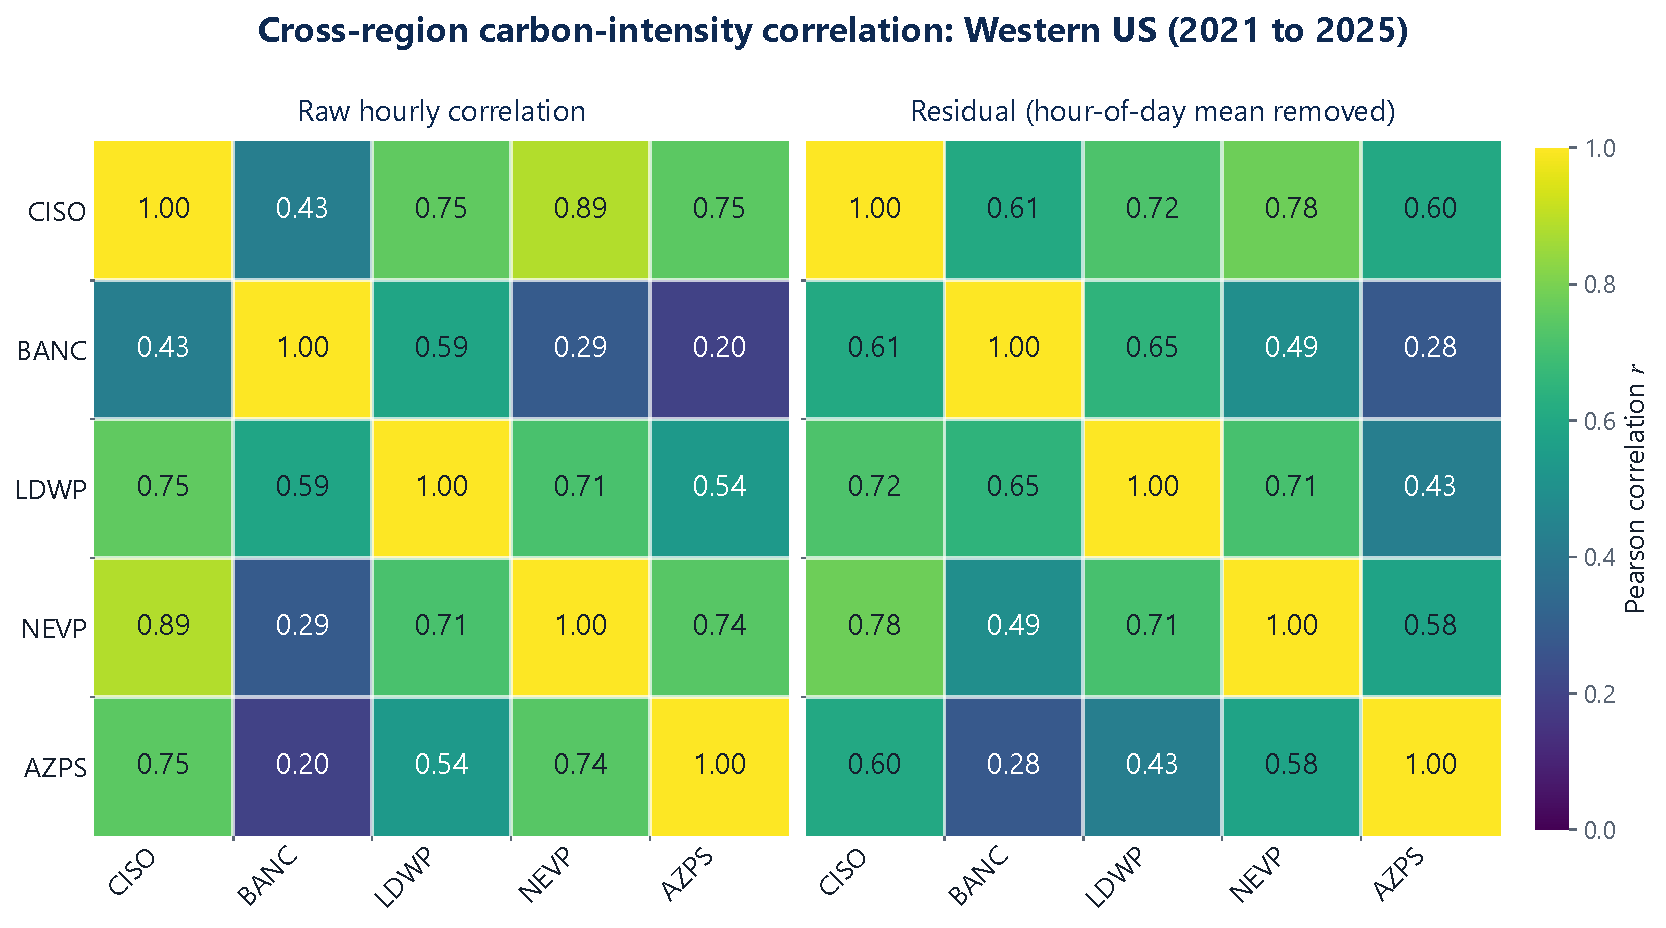
\includegraphics[width=0.48\textwidth]{../figures/ci_corr_heatmap_us_west.pdf}\hfill
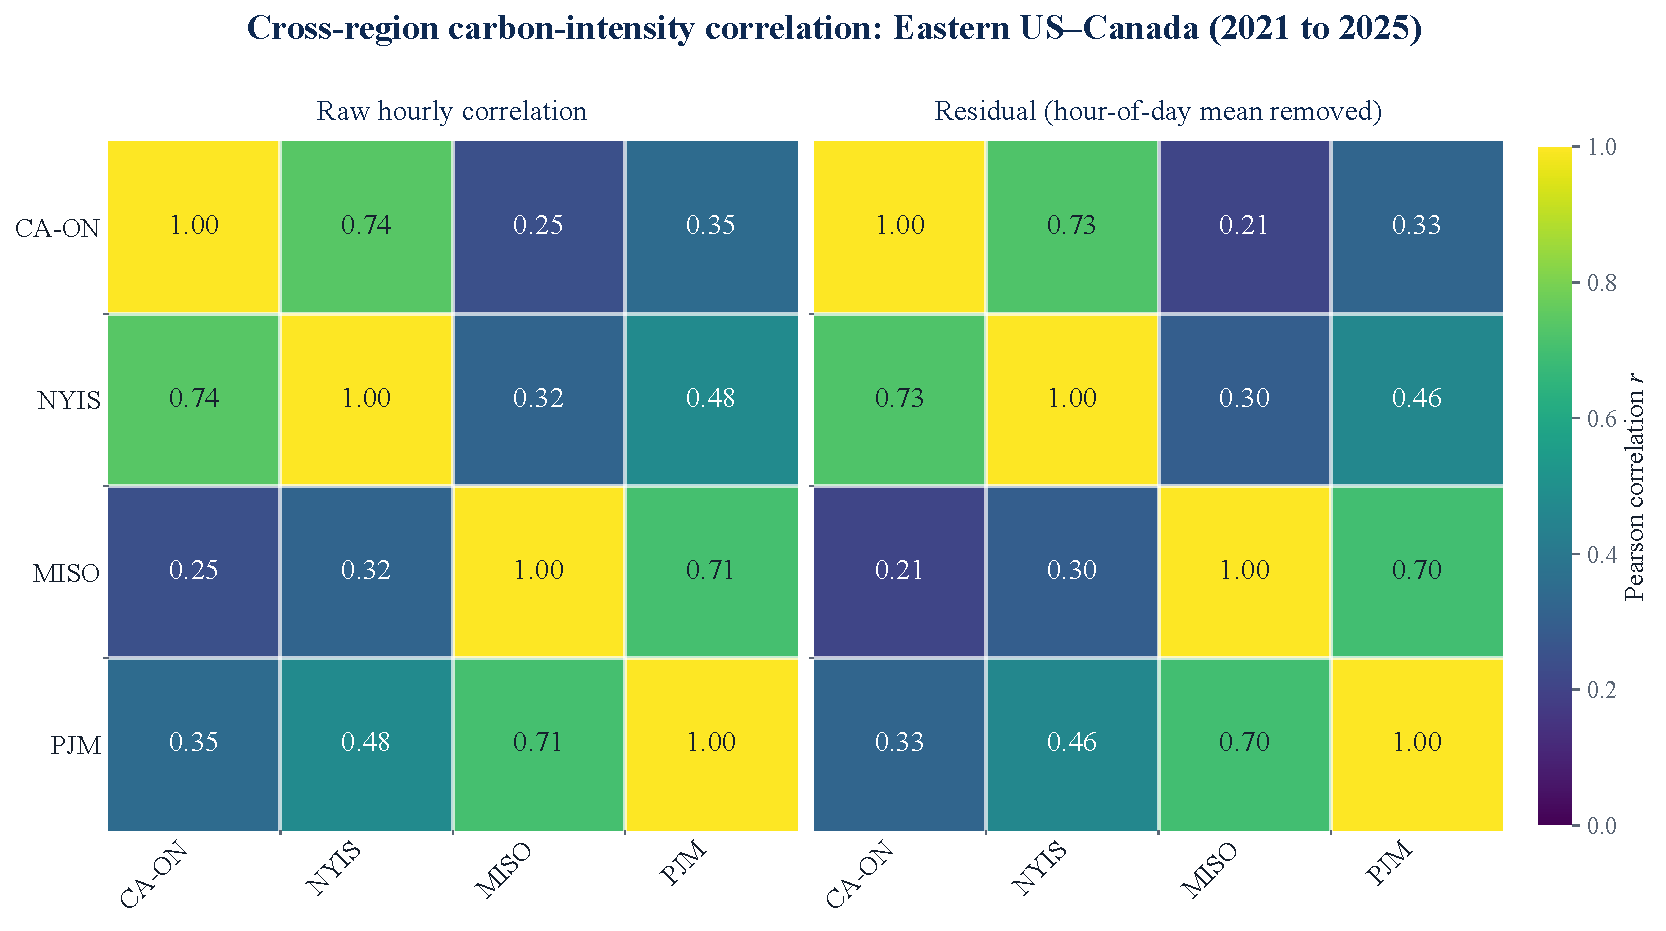
\includegraphics[width=0.48\textwidth]{../figures/ci_corr_heatmap_taskc.pdf}
\caption{Residual (hour-of-day-removed) cross-region correlation of hourly carbon
intensity, 2021--2025. Left: US West (CISO, BANC, LDWP, NEVP, AZPS). Right:
Ontario--Eastern belt (CA-ON, NYISO, MISO, PJM). Spatial correlation is strong and
genuine in both --- the assumption motivating spatial DRO is empirically valid.}
\label{fig:heatmaps}
\end{figure}

\subsection{The spatial gap is null across the spectrum (RQ2)}\label{sec:res-gap}
Table~\ref{tab:gaps} reports the spatial gap \eqref{eq:gap} for the three
pre-registered US/Canada cases: nine cells each (three constraint regimes $\times$
three $\alpha$-levels), CV-selected $\varepsilon^\star$, single test read on 2025.
The gap never exceeds a few tenths of one percent of test
$\CVaR_{0.95}$ in either direction, and where the bootstrap calls a cell
``detectable'' the signs flip across adjacent $\alpha$-levels --- the signature of
solver-path artifacts rather than exploitable structure. The California/Nevada
panel agrees (gaps in $[-0.012,+0.058]\%$, DRO active throughout).

Crucially, this is a null of the \emph{strong} kind. In all three pre-registered
cases cross-validation \emph{chooses} a non-trivial ambiguity radius:
$\varepsilon^\star=1$ in every one of the 27 cells for \texttt{taskc} and
\texttt{us\_hetero}, and in 25 of 27 for \texttt{us\_west}. The DRO is therefore
genuinely engaged --- it is paying for robustness, not collapsing to the nominal
problem --- and the two arms still coincide. A null in which CV had selected
$\varepsilon^\star=0$ would be uninformative (robustification switched off, so the
arms must match by construction); here the robustification is demonstrably on and
the spatial covariance still buys nothing. This is the first regime in the project
where the DRO is consistently active, which is precisely what makes the null
informative rather than vacuous.

The Iberia--France panel is the instructive contrast and the project's historical
starting point. There the residual correlation is near zero, and CV does not even
consistently engage the DRO: $\varepsilon^\star$ flickers between $0$, $0.1$, $1$
and $10$ across cells, collapsing to $0$ in several. This is itself consistent with
the thesis --- where there is no cross-region structure, the machinery sees nothing
worth robustifying --- but it makes the Iberian null the \emph{weak} kind. We
therefore retain it only as low-correlation, real-grid external validity, and rest
the central claim on the US/Canada cases where the DRO is unambiguously on. The
engineered \texttt{us\_hetero} portfolio supplies the strong zero-correlation null
($\varepsilon^\star=1$ throughout, still no value) that Iberia cannot.

\begin{table}[t]
\centering\small
\caption{Spatial gap (\% of test $\CVaR_{0.95}$; positive $=$ joint covariance
better) for the three US/Canada cases. R3 $=$ reference regime, R1 $=$ $+$deadline,
R2 $=$ $+$variable carbon-coupled capacity. ``det.''\ $=$ bootstrap 95\% CI
excludes zero.}
\label{tab:gaps}
\begin{tabular}{llrrrrrr}
\toprule
& & \multicolumn{2}{c}{\texttt{us\_hetero} ($\bar r\approx0$)} &
\multicolumn{2}{c}{\texttt{taskc} ($\bar r\approx0.5$)} &
\multicolumn{2}{c}{\texttt{us\_west} ($\bar r\approx0.5$)}\\
\cmidrule(lr){3-4}\cmidrule(lr){5-6}\cmidrule(lr){7-8}
Regime & $\alpha$ & gap\,\% & det. & gap\,\% & det. & gap\,\% & det.\\
\midrule
R3 & 0.30 & $-0.233$ & \checkmark & $-0.022$ & \checkmark & $+0.043$ & \\
R3 & 0.50 & $-0.177$ & \checkmark & $-0.002$ &  & $+0.032$ & \\
R3 & 0.75 & $+0.001$ &  & $+0.034$ & \checkmark & $-0.005$ & \\
R1 & 0.30 & $-0.233$ & \checkmark & $-0.022$ & \checkmark & $+0.014$ & \\
R1 & 0.50 & $-0.177$ & \checkmark & $-0.002$ &  & $+0.028$ & \\
R1 & 0.75 & $+0.001$ &  & $+0.034$ & \checkmark & $+0.002$ & \\
R2 & 0.30 & $-0.211$ & \checkmark & $+0.038$ & \checkmark & $+0.008$ & \\
R2 & 0.50 & $-0.154$ & \checkmark & $+0.030$ & \checkmark & $+0.005$ & \\
R2 & 0.75 & $+0.062$ & \checkmark & $+0.009$ &  & $+0.000$ & \checkmark\\
\bottomrule
\end{tabular}
\end{table}

Three readings of Table~\ref{tab:gaps} matter. First, in the adversarial
diversification case (\texttt{us\_hetero}) the joint covariance actually
\emph{hurts} at low $\alpha$ (up to $-0.23\%$): with no true cross-structure, the
joint estimator fits noise that the block-diagonal arm is spared. Second, in the
strongly correlated belt (\texttt{taskc}) the detectable cells flip sign between
$\alpha=0.30$ and $\alpha=0.75$ within the same regime. Third, the US West ---
strongest correlation of all --- produces no detectable cell beyond one of
magnitude $+3\times10^{-6}\%$. Figure~\ref{fig:finding}A plots all 27 cells
against each case's mean residual correlation: the cloud stays on zero across the
whole correlation range. \textbf{Validity of the spatial assumption does not imply
value from it.}

\begin{figure}[t]
\centering
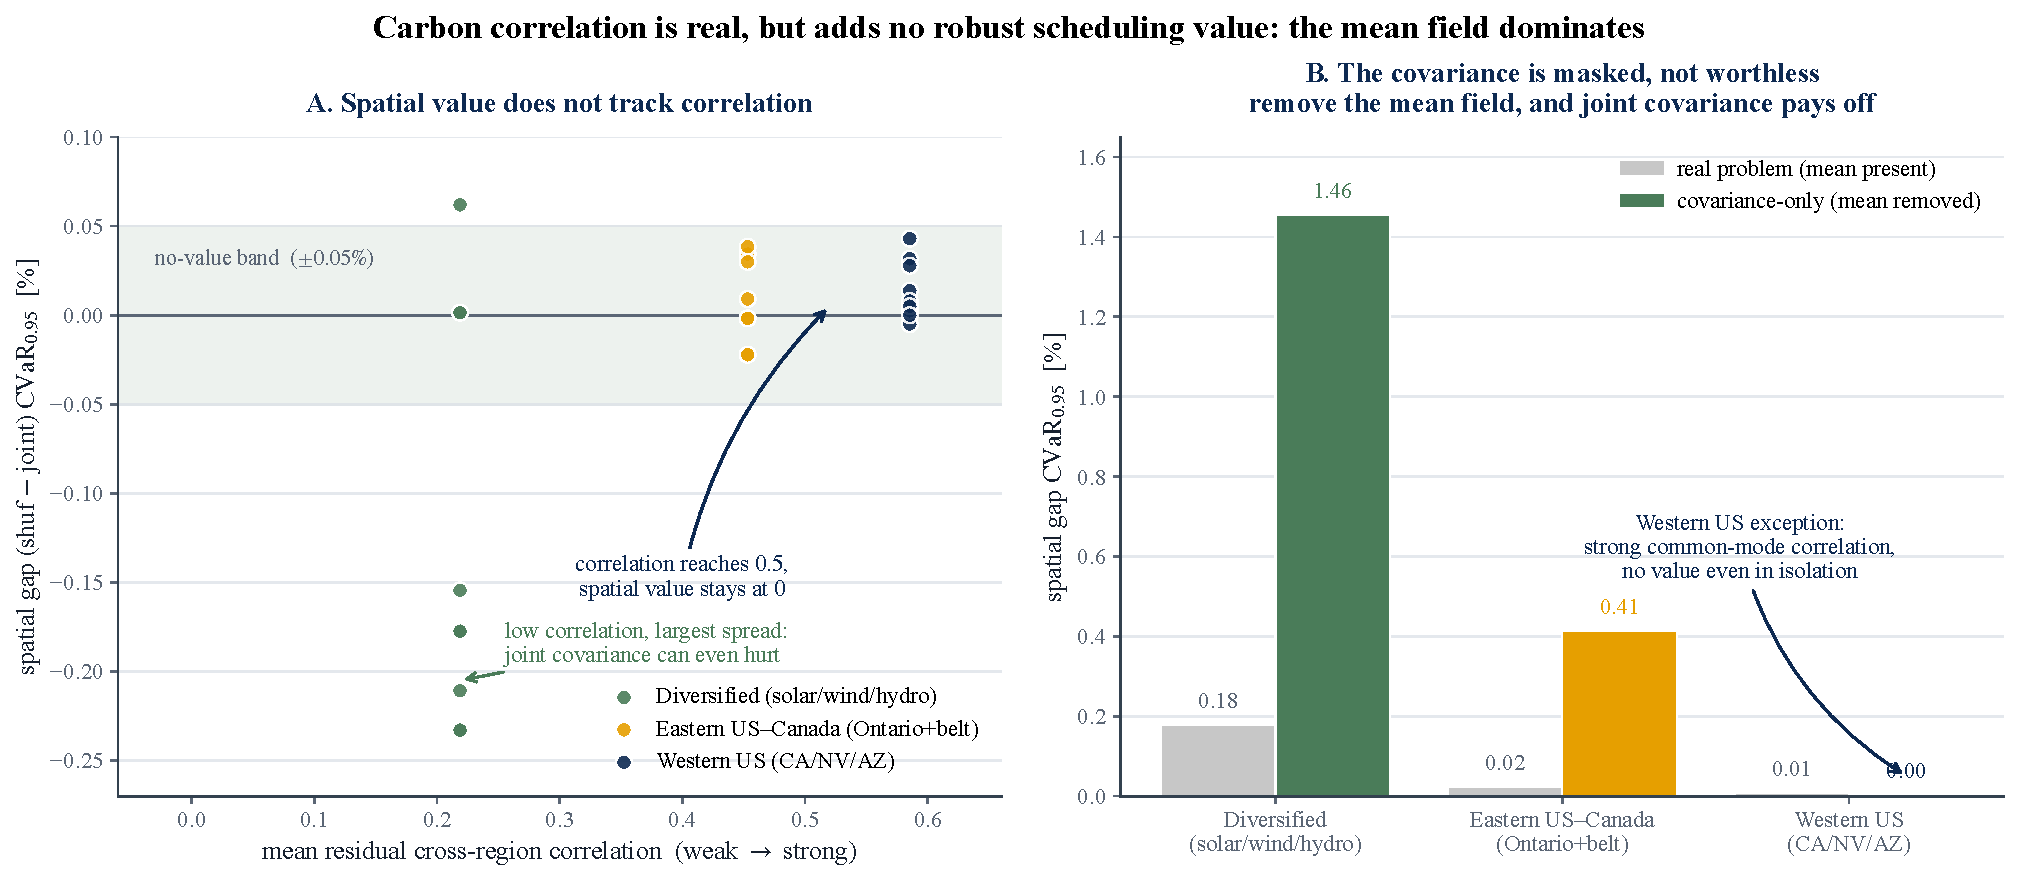
\includegraphics[width=\textwidth]{../figures/finding.pdf}
\caption{The Phase 1 finding. \textbf{A:} spatial gap vs.\ mean residual
cross-region correlation --- value does not track correlation anywhere on the
spectrum. \textbf{B:} mean-ablation --- in the covariance-only world (constant
scheduling mean) the joint covariance pays off by up to $+1.46\%$, proving the
spatial signal is real but \emph{masked} by the mean carbon field, not absent.}
\label{fig:finding}
\end{figure}

\subsection{The null survives a pre-registered robustness battery
(RQ2)}\label{sec:res-robust}
Table~\ref{tab:robust} summarizes. Re-estimating the covariance with Ledoit--Wolf
shrinkage, seasonal residuals, or AR(1) residuals never produces a spatial effect
that passes the pre-registered agreement rule (positive and sign-stable across
both residual estimators). The largest battery value anywhere, $+0.179\%$ (AR(1),
\texttt{taskc}, $\alpha=0.30$), appears \emph{only} under AR(1) and not under the
seasonal estimator, so the rule rejects it. Benjamini--Hochberg correction at
$q=0.05$ across all 144 non-ablation cells leaves that same already-rejected cell
as the largest surviving positive gap --- nothing material survives both filters.
A walk-forward refit (train 2021--2023, test 2024) reproduces the null out of
time: maximum absolute gap $0.036\%$ (\texttt{taskc}), $0.028\%$
(\texttt{us\_west}), $0.217\%$ (\texttt{us\_hetero}, again negative). An
11-point log-denser $\varepsilon$ grid changes no gap at the reported precision.
Finally, a \emph{constraint-tightness} sensitivity directly probes the most
plausible route to spatial value: tripling the binding tightness of the ramp limit
($\Delta_r=5$ instead of $15$ MW/h) shrinks the feasible set so the schedule has far
less freedom to track the mean field --- yet the null is unmoved, with maximum
absolute gap $0.028\%$ (\texttt{us\_west}), $0.044\%$ (\texttt{taskc}) and $0.169\%$
(\texttt{us\_hetero}), all sign-flipping and with $\varepsilon^\star=1$ retained.
The covariance does not begin to pay even when the mean's pull is mechanically
curtailed.

\begin{table}[t]
\centering\small
\caption{Robustness battery: maximum $|$gap$|$ (\%) per covariance estimator, and
temporal walk-forward (test year 2024). No cell passes the pre-registered
agreement rule (positive and sign-stable under both seasonal and AR(1)
residualization).}
\label{tab:robust}
\begin{tabular}{lrrrr}
\toprule
Case & Ledoit--Wolf & Seasonal & AR(1) & Walk-forward 2024\\
\midrule
\texttt{us\_hetero} & 0.233 & 0.355 & 0.035 & 0.217\\
\texttt{taskc}      & 0.037 & 0.034 & 0.179 & 0.036\\
\texttt{us\_west}   & 0.043 & 0.066 & 0.017 & 0.028\\
\bottomrule
\end{tabular}
\end{table}

\subsection{Mean-ablation: the covariance is masked, not worthless
(RQ3)}\label{sec:res-ablation}
The ablation isolates the cause (Table~\ref{tab:ablation},
Figure~\ref{fig:finding}B). Under \textsc{level} ablation --- regional
time-averages equalized, hour-of-day shape kept --- every gap is unchanged to
three decimals: the \emph{between-region} mean differences are not what masks the
covariance. Under \textsc{flat} ablation --- constant scheduling mean, the
covariance-only world --- the joint covariance suddenly pays: up to $+1.46\%$ in
\texttt{us\_hetero} and $+0.41\%$ in \texttt{taskc}, all BH-significant, and CV no
longer collapses both arms onto the same schedule. The spatial signal in the
covariance is therefore \emph{real and exploitable}; in the real problem it is
simply dominated by the within-day shape of the mean carbon field, which both arms
share. The instructive exception is \texttt{us\_west}: even in the covariance-only
world its gaps stay at zero ($-0.036$ to $+0.004\%$), because its strong
correlation is \emph{common-mode} --- all five zones move together, so destroying
cross-dependence changes no scheduling decision. Positive correlation is
non-diversifiable risk: there is no hedge for a DRO to find.

\begin{table}[t]
\centering\small
\caption{Mean-ablation: spatial gap range (\%) across the nine cells per case.
\textsc{level} (equalize regional time-averages) leaves the null untouched;
\textsc{flat} (constant scheduling mean $=$ covariance-only world) reveals genuine
spatial value except where correlation is common-mode (\texttt{us\_west}).}
\label{tab:ablation}
\begin{tabular}{lccc}
\toprule
Case & Real problem & \textsc{level} & \textsc{flat} (covariance-only)\\
\midrule
\texttt{us\_hetero} & $-0.233\ldots+0.062$ & unchanged & $+0.39\ldots+1.46$\\
\texttt{taskc}      & $-0.022\ldots+0.038$ & unchanged & $+0.14\ldots+0.41$\\
\texttt{us\_west}   & $-0.005\ldots+0.043$ & unchanged & $-0.04\ldots+0.00$\\
\bottomrule
\end{tabular}
\end{table}

\subsection{Tail dependence: the structure is non-elliptical
(RQ3)}\label{sec:res-tails}
Table~\ref{tab:tails} reports residual tail-dependence at $q=0.95$ for
representative pairs. Two findings. \emph{First}, the upper tail is empirically at
or below the Gaussian benchmark everywhere (excess $-0.18$ to $+0.04$): in the
dirtiest hours, regions \emph{de-couple} rather than spike together --- there is
no upper-tail co-movement for a richer ambiguity set to exploit on the risk side.
\emph{Second}, the dependence is radially asymmetric, $\chiL>\chiU$: regions go
\emph{clean} together more strongly than dirty together, clearest in the
solar-driven US West (CISO--LDWP $\chiL=0.48$ vs.\ $\chiU=0.25$; BANC--LDWP $0.40$
vs.\ $0.17$). Elliptical copulas force $\chiL=\chiU$, so this is structure a
Mahalanobis--Wasserstein ball is geometrically incapable of representing --- the
covariance is not merely masked (Section~\ref{sec:res-ablation}); for the part of
the dependence that varies, it is also the \emph{wrong object}.
Figure~\ref{fig:tails} shows the asymmetry for the Ontario--Eastern belt.

\begin{figure}[t]
\centering
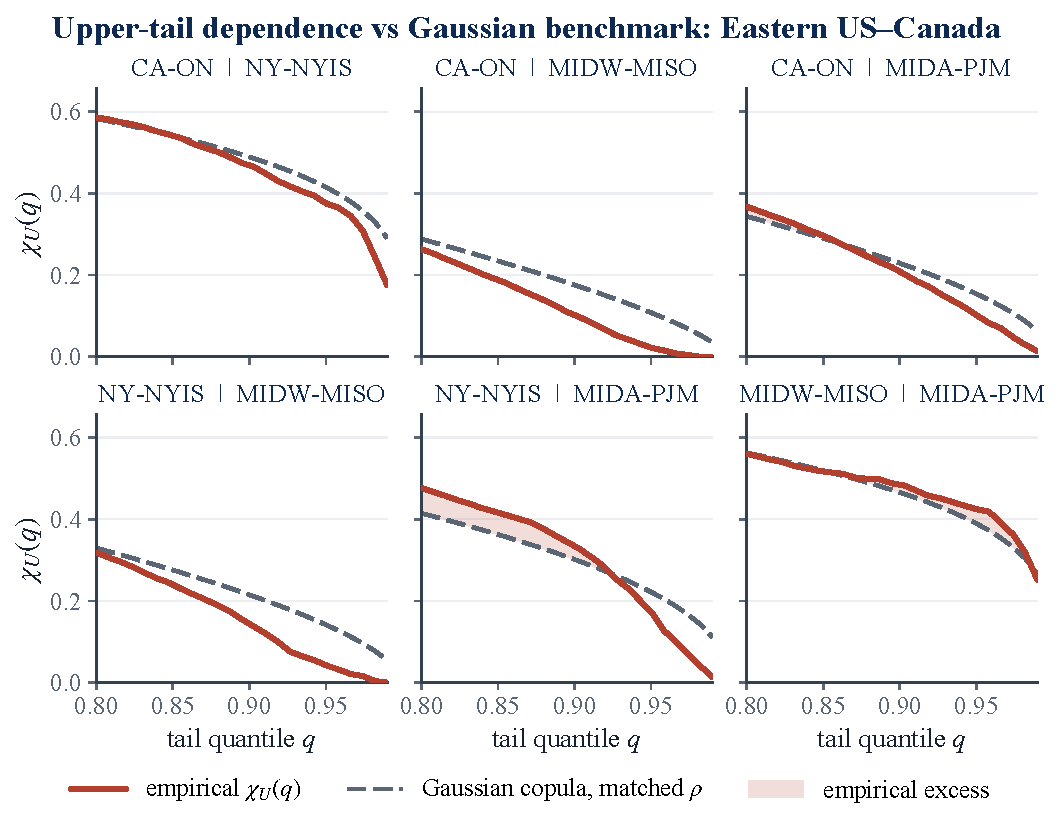
\includegraphics[width=0.72\textwidth]{../figures/tail_dependence_taskc.pdf}
\caption{Upper-tail dependence $\chiU(q)$ for the Ontario--Eastern belt region
pairs (solid) against the Gaussian-copula benchmark at the matched correlation
(dashed). The empirical curves sit at or below the benchmark as $q\to1$: in the
dirtiest hours the regions decouple, so there is no exploitable upper-tail
co-movement for a richer ambiguity set to capture. The complementary radial
asymmetry ($\chiL>\chiU$) is quantified in Table~\ref{tab:tails}.}
\label{fig:tails}
\end{figure}

\begin{table}[t]
\centering\small
\caption{Residual tail dependence at $q=0.95$ for selected pairs. ``Excess'' $=$
empirical $\chiU$ minus the Gaussian-copula value at the matched correlation
$\rho$. Throughout, $\chiU$ shows no exploitable upper-tail excess while
$\chiL>\chiU$ signals non-elliptical (radially asymmetric) dependence.}
\label{tab:tails}
\begin{tabular}{llccccc}
\toprule
Case & Pair & $\rho$ & $\chiU$ emp & $\chiU$ Gauss & Excess & $\chiL$ emp\\
\midrule
\texttt{us\_west} & CISO--LDWP & 0.72 & 0.25 & 0.41 & $-0.16$ & 0.48\\
\texttt{us\_west} & BANC--LDWP & 0.65 & 0.17 & 0.35 & $-0.18$ & 0.40\\
\texttt{us\_west} & CISO--NEVP & 0.78 & 0.43 & 0.47 & $-0.05$ & 0.39\\
\texttt{taskc} & CA-ON--NYISO & 0.73 & 0.38 & 0.42 & $-0.04$ & 0.31\\
\texttt{taskc} & MISO--PJM    & 0.70 & 0.43 & 0.39 & $+0.04$ & 0.42\\
\texttt{us\_hetero} & CISO--BPAT & 0.33 & 0.10 & 0.16 & $-0.06$ & 0.26\\
\texttt{us\_hetero} & ERCOT--BPAT & 0.00 & 0.04 & 0.05 & $-0.02$ & 0.02\\
\bottomrule
\end{tabular}
\end{table}

\subsection{Phase 2: the null survives richer dependence models
(RQ3)}\label{sec:res-copula}
If the covariance ball failed only because it is elliptical, a copula that encodes
the empirical $\chiL>\chiU$ asymmetry should recover value. It does not.
Figure~\ref{fig:copuladens} confirms the Clayton copula fitted to each grid behaves
as intended --- its samples pile into the joint-clean corner ($\chiL=0.70$ vs.\
$\chiU=0.26$ for CISO--BANC), exactly the structure the symmetric Gaussian copula
($\chiL\approx\chiU\approx0.46$) and any covariance ball cannot represent. Yet when
each dependence model is used to schedule and evaluated out-of-sample on 2025
(Table~\ref{tab:copula}, Figure~\ref{fig:copularesult}), no fitted copula beats the
independence baseline by a material, sign-stable margin; the Gaussian and Clayton
gains never exceed $0.16\%$ of $\CVaR_{0.95}$ and flip sign across $\alpha$ exactly
as in Phase 1.

To test the \emph{actual} worst case we add the comonotone (upper-Fr\'echet) arm:
perfect rank coupling, which maximizes the CVaR of a sum of positively-associated
risks and therefore realizes the supremum $\sup_C$ in the leverage $\Lambda$ of
Section~\ref{sec:method-copula}. This is the most any copula can buy. In the two
weakly- or heterogeneously-coupled grids it too returns nothing sign-stable
($\le0.11\%$, not detectable). In the genuinely positively-coupled belt
(\texttt{taskc}, $\bar\tau=0.31$) it does produce a sign-stable, fully-detectable
gain --- but of only $+0.10$ to $+0.18\%$ across all nine cells. This is the key
number: the comonotone arm \emph{measures} the copula ceiling directly, and even
perfect knowledge of the dependence caps the achievable gain at
$\Lambda\approx0.18\%$ of $\CVaR_{0.95}$ --- immaterial, and an order of magnitude
below the schedule's mean-driven value. Crucially this measurement is
\emph{independent} of the mean-ablation, so it pins $\Lambda$ without circularity:
no copula, not even the maximal one, recovers material value.

\begin{figure}[t]
\centering
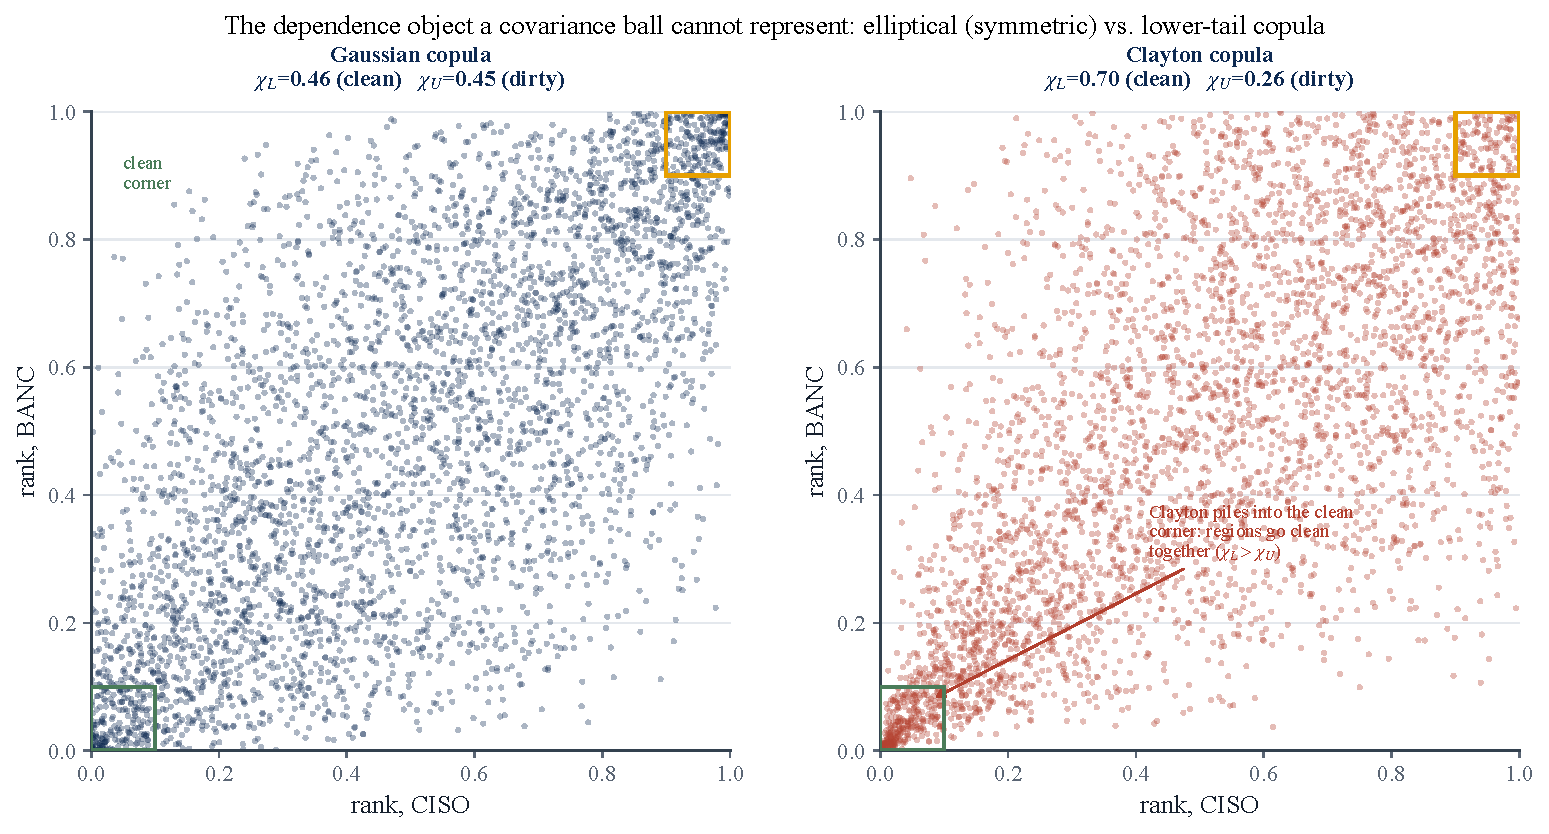
\includegraphics[width=\textwidth]{../figures/copula_density.pdf}
\caption{The dependence object a covariance ball cannot represent. Samples from the
Gaussian copula (left, symmetric: $\chiL\approx\chiU$) and the fitted Clayton copula
(right) for a representative US-West pair. Clayton concentrates in the lower-left
``clean'' corner ($\chiL>\chiU$), reproducing the Phase 1 radial asymmetry that
elliptical models force to zero.}
\label{fig:copuladens}
\end{figure}

\begin{table}[t]
\centering\small
\caption{Phase 2 copula results. Gap $=$ reduction in out-of-sample
$\CVaR_{0.95}$ versus the independence baseline (\%; positive $=$ the copula helps),
reported as the maximum \emph{positive} gain over the nine cells. The
\emph{comonotone} arm is the upper Fr\'echet bound (perfect rank coupling) --- the
supremum over all copulas, hence the empirical ceiling $\Lambda$ on copula value.
$\theta$ is the fitted Clayton parameter; ``stable'' flags a sign-stable,
bootstrap-detectable gain across all nine cells.}
\label{tab:copula}
\begin{tabular}{lccccccc}
\toprule
Case & $\bar\tau$ & $\theta$ & gain$_{\text{Gauss}}$ & gain$_{\text{Clay}}$ &
gain$_{\text{comon}}$ & $\Lambda$ stable? & material?\\
\midrule
\texttt{us\_west}   & 0.47 & 1.77 & 0.066 & 0.038 & 0.089 & no & no\\
\texttt{taskc}      & 0.31 & 0.90 & 0.158 & 0.014 & 0.182 & \textbf{yes (9/9)} & no\\
\texttt{us\_hetero} & 0.20 & 0.50 & 0.069 & 0.127 & 0.114 & no & no\\
\bottomrule
\end{tabular}
\end{table}

\begin{figure}[t]
\centering
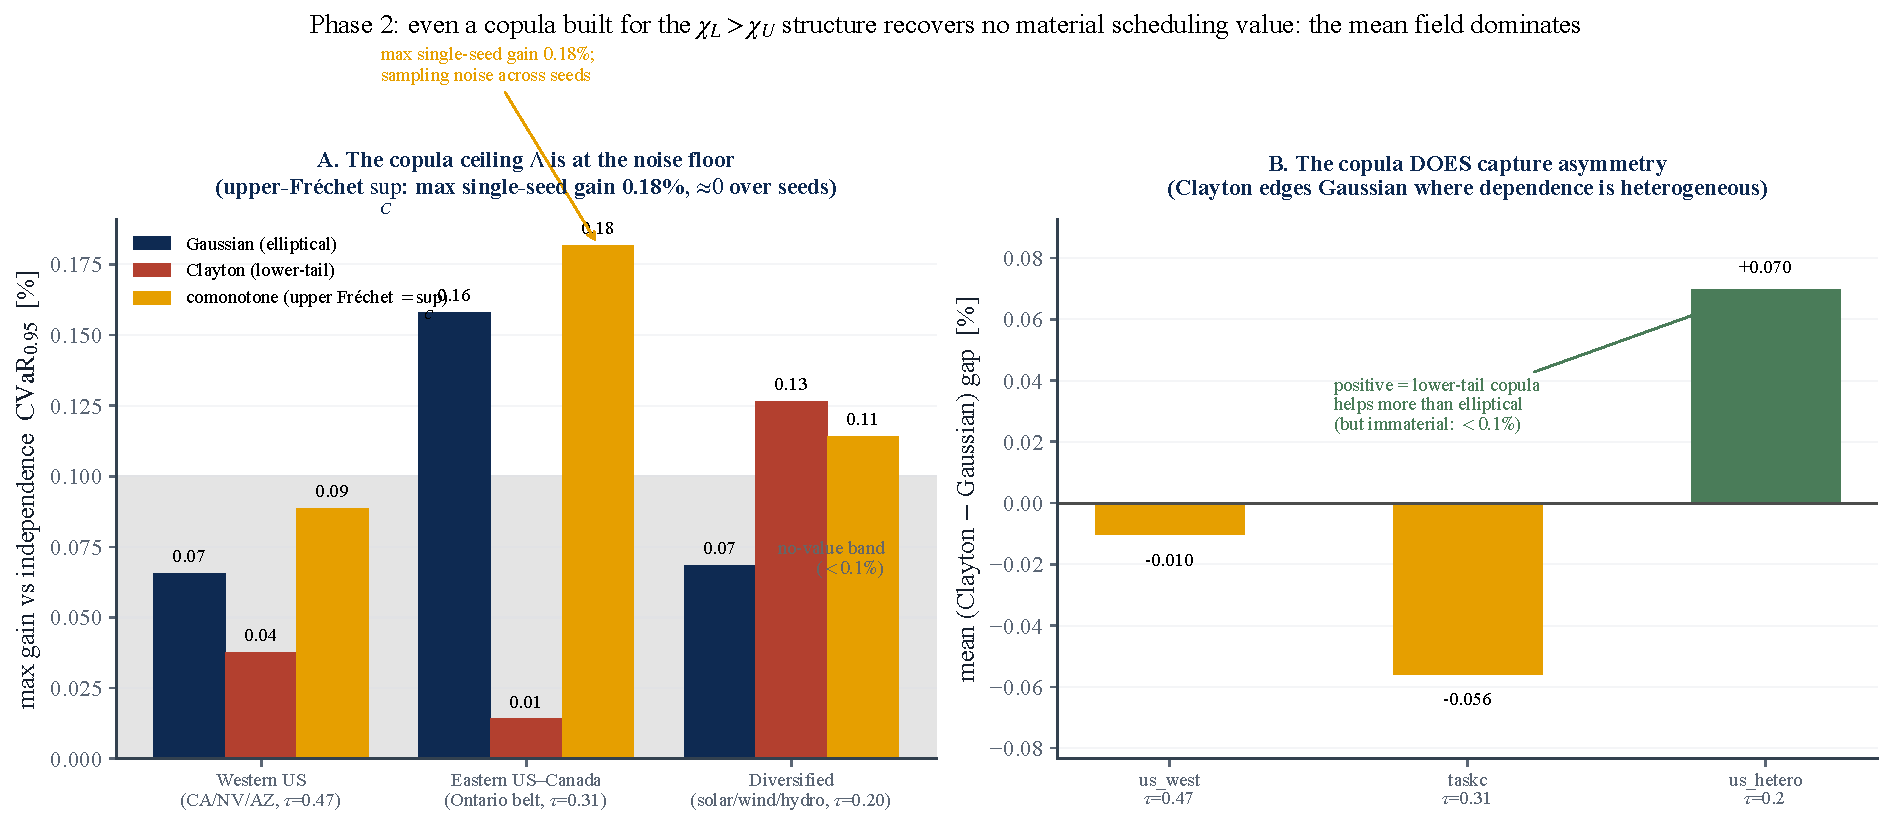
\includegraphics[width=\textwidth]{../figures/copula_result.pdf}
\caption{Phase 2 result. \textbf{A:} maximum positive gain versus independence for
the Gaussian, Clayton, and comonotone (upper-Fr\'echet $\sup_C$) arms. The
comonotone ceiling $\Lambda$ caps at $0.18\%$, and only in the coupled belt
(\texttt{taskc}); the fitted copulas do not even reach it. \textbf{B:} the mean
Clayton$-$Gaussian increment by grid; positive where dependence is heterogeneous
(\texttt{us\_hetero}, $+0.07\%$), confirming the copula \emph{does} capture the
asymmetry --- but an order of magnitude too small to matter, as
Proposition~\ref{prop:meandom} predicts.}
\label{fig:copularesult}
\end{figure}

One positive signal is worth stating precisely: the Clayton$-$Gaussian increment is
consistently positive in the heterogeneous case (\texttt{us\_hetero}, mean
$+0.07\%$) and negligible or negative where correlation is common-mode. The
asymmetric copula therefore \emph{does} extract something the elliptical one cannot,
in the expected direction --- but at a magnitude an order below materiality. This is
the empirical face of Proposition~\ref{prop:meandom}: the copula's leverage
$\Lambda$ is real but dominated by the mean field. Phase 2 thus converts the Phase 1
null from ``covariance is the wrong object'' into the stronger ``\emph{no} dependence
model recovers value here, because the binding constraint is the mean field, not the
shape of the dependence.''

% ===================== 5. DISCUSSION (RUN 2) =====================
\section{Discussion}\label{sec:discussion}

\subsection{What the null means, and what it does not}
The result is a \emph{specification} finding, not a failure of carbon-aware
scheduling. Carbon intensity \emph{is} spatially correlated where the literature
expects it to be (Section~\ref{sec:res-corr}), and the DRO machinery \emph{is}
active (CV selects $\varepsilon^\star=1$ almost everywhere). What the experiment
falsifies is the specific hypothesis that encoding that correlation in a
covariance-based ambiguity set improves robust scheduling. The mean-ablation
result (Section~\ref{sec:res-ablation}) is what licenses the stronger claim: the
covariance signal is genuine and, in a covariance-only world, worth up to
$1.46\%$ of tail emissions --- it is simply dominated by the diurnal mean carbon
field in the problem as actually posed. A reader could otherwise dismiss the null
as ``the data had no signal''; the ablation shows the signal is present but
\emph{subordinate}. This is the central intellectual contribution: a clean
separation of \emph{validity} of a modelling assumption from its \emph{value}.

\subsection{Why the mean dominates: a mechanism}
Three forces compound. (i)~\emph{Magnitude.} The within-day swing of mean carbon
intensity (night-to-noon ratios of two-to-fourfold in solar-heavy grids) dwarfs
the residual covariance, so the optimal schedule is driven almost entirely by
\emph{when} each region is clean on average; the second-order covariance term
moves decisions only at the margin. (ii)~\emph{Common-mode correlation.} Where
correlation is strongest (US West), it is positive and shared across all zones ---
common, non-diversifiable risk. Diversification value requires \emph{offsetting}
fluctuations; positively co-moving regions offer no hedge, so destroying the
cross-blocks (the shuffled arm) changes nothing. (iii)~\emph{Wrong tail.} Robust
\emph{tail} scheduling cares about joint \emph{dirty} excursions, but the empirical
upper tail is independent-to-decoupling ($\chiU$ at or below Gaussian), while the
co-movement that does exist is in the \emph{clean} tail ($\chiL>\chiU$) --- exactly
the regime a risk-averse scheduler is not protecting against, and a radial
asymmetry an elliptical ball cannot encode regardless. The covariance is thus both
\emph{masked} (dominated by the mean) and, for its varying part, \emph{mis-shaped}
(non-elliptical).

\subsection{Relation to prior work}
The finding refines rather than contradicts the carbon-aware DRO literature.
Single-region robust formulations~\citep{wijayawardana2025} remain well-motivated:
our per-region marginal schedulers capture essentially all the value. The
contribution is to the \emph{multi-region} extension that treats carbon intensity
as a correlated vector --- a natural and previously untested generalization. We
show that the covariance channel of that extension is empirically inert under
realistic grid data, and we locate the reason in the mean-dominance and
non-ellipticity of the dependence. This both saves practitioners from modelling
complexity that does not pay and gives theorists a precise target: the value, if
any, lives in non-elliptical tail structure that a Wasserstein ball over
covariance cannot reach.

\subsection{Practical recommendation}
For carbon-aware schedulers on the grids studied, a \emph{per-region marginal}
robust scheduler --- one ambiguity set per zone, no cross-region covariance ---
captures essentially all the achievable robust value at a fraction of the
modelling and estimation cost. Estimating a full joint covariance is not merely
unnecessary; in the diversification-friendly case it is mildly
\emph{counterproductive} (the joint arm fit noise and \emph{lost} up to $0.23\%$).
The engineering effort spared by not modelling spatial covariance is better spent
on accurate per-region mean forecasts, which is where the value demonstrably lies.

\subsection{Limitations}
Five bound the claims. \emph{(i)~Representative schedule.} We evaluate one
canonical workload (fixed daily utilization, splittable load, ramp limits). A
sharply different cost geometry could in principle re-weight the covariance term;
the constraint-tightness sensitivity (Section~\ref{sec:res-robust}) addresses the
most plausible case --- a $3\times$ tighter ramp leaves the null intact --- but a
qualitatively different objective (e.g.\ hard per-job deadlines) is untested.
\emph{(ii)~Test horizon.} The primary read is a single held-out year (2025);
walk-forward to 2024 reproduces the null, but multi-year rolling evaluation would
strengthen external validity. \emph{(iii)~Dependence model.} The DRO uses a
covariance (second-moment) ambiguity set by construction; Phase 2
(Section~\ref{sec:res-copula}) closes this gap with Gaussian and Clayton copula
schedulers, but a full copula-\emph{ambiguity} Wasserstein DRO in the
Fan--Ji--Lejeune sense remains future work. \emph{(iv)~Geographic scope.} The region sets span WECC, the
Eastern Interconnection, and Iberia--France across the dependence spectrum, but
grids with different generation mixes (e.g.\ hydro-thermal systems with strong
seasonal storage) remain untested. \emph{(v)~Data licence and clocks.} Carbon
intensity is Electricity Maps lifecycle estimates on a common local clock per
region set; alternative intensity methodologies or clock conventions could shift
point estimates, though not by the order of magnitude separating the observed gaps
from materiality.

% ===================== 6. CONCLUSIONS (RUN 3) =====================
\section{Conclusions}\label{sec:conclusion}

\subsection{Answers to the research questions}
\textbf{RQ1 --- Is carbon intensity spatially correlated in coupled grids?}
Yes. After removing the shared diurnal cycle, residual cross-region correlations
reach $0.78$ in the US West and $0.73$ in the Ontario-anchored Eastern belt and
survive de-seasonalization (Section~\ref{sec:res-corr}). The premise of spatial
DRO is empirically sound; the engineered heterogeneous portfolio confirms the
diagnostic resolves genuine near-zero dependence ($0.00$) when it is present.

\textbf{RQ2 --- Does encoding that correlation in a covariance-based ambiguity set
improve robust scheduling?} No. Across three primary region sets spanning the
dependence spectrum (and two corroborating panels), the out-of-sample
$\CVaR_{0.95}$ spatial gap never exceeds a few tenths
of one percent and is not sign-stable; the null survives Ledoit--Wolf shrinkage,
seasonal and AR(1) residualization, Benjamini--Hochberg correction over 144 cells,
walk-forward validation to 2024, and a log-denser $\varepsilon$ grid
(Sections~\ref{sec:res-gap}--\ref{sec:res-robust}). In the most
diversification-friendly case the joint covariance is mildly counterproductive.
Critically, this is an \emph{active} null: cross-validation selects a non-trivial
ambiguity radius ($\varepsilon^\star=1$) in nearly every cell of the US/Canada
cases, so the DRO is genuinely robustifying and the spatial covariance still adds
nothing --- a stronger result than a null in which the robustification had
collapsed to the nominal problem.

\textbf{RQ3 --- Why?} Two complementary mechanisms. A mean-ablation experiment
proves the covariance signal is real and worth up to $1.46\%$ of tail emissions in
a covariance-only world, but is dominated by the diurnal mean carbon field in the
problem as posed (Section~\ref{sec:res-ablation}). A tail-dependence analysis shows
the residual dependence is non-elliptical --- upper-tail-independent and radially
asymmetric ($\chiL>\chiU$) --- and therefore structurally invisible to a
covariance ball even where it does vary (Section~\ref{sec:res-tails}). The
covariance is both \emph{masked} and \emph{mis-shaped}. Phase 2 settles which
mechanism binds: replacing the covariance ball with a Clayton copula built for the
$\chiL>\chiU$ asymmetry still recovers no material value
(Section~\ref{sec:res-copula}), and Proposition~\ref{prop:meandom} explains why ---
CVaR's translation invariance makes the dependence model second-order to the mean
field. The limit is not the shape of the dependence object; it is mean-dominance.

\subsection{Contributions}
This thesis contributes: (1)~a pre-registered falsification methodology
(shuffled-marginals, extended to copula-coupled resampling) that cleanly separates
the \emph{validity} of a spatial modelling assumption from its \emph{value},
transferable to any correlated-uncertainty DRO; (2)~a replicated,
robustness-checked null on whether spatial dependence improves carbon-aware DRO
scheduling, holding across multiple real grids \emph{and} across the dependence
hierarchy from covariance ball to elliptical and lower-tail copulas;
(3)~a causal mechanism --- formalized as a mean-dominance bound
(Proposition~\ref{prop:meandom}) and demonstrated by mean-ablation --- that
explains the null rather than merely reporting it; and (4)~a fully reproducible,
version-controlled, CI-tested pipeline (168 tests) with archived license-safe
summary tables for every reported number.

\subsection{Future work}
Phase 2 closed the most immediate question --- whether a copula that sees the
asymmetry recovers value (it does not) --- and in doing so sharpened the remaining
agenda. First, a \emph{copula-ambiguity Wasserstein DRO} in the Fan--Ji--Lejeune
sense \citep{fan2024}, which robustifies the dependence structure itself rather than
sampling from a single fitted copula; Proposition~\ref{prop:meandom} predicts the
mean field will still dominate, but this would make the claim fully model-free.
Second, an \emph{inter-region transfer channel}: allowing load to physically
migrate between zones ($f_{r\to s,t}$) converts spatial structure from a passive
hedge into an active decision lever and remains an SOCP; because the mean-dominance
bound concerns \emph{passive} risk reduction, the transfer channel is the most
promising route to extracting spatial value, and it overlaps a collaborator's scope
pending supervisor sign-off. Third, \emph{rolling re-optimization} over multiple
test years. The null is thus not a dead end but a sharpened mandate: it shows that
the value, if any, will not come from a better passive dependence model but from an
active spatial decision.

% ===================== REFERENCES =====================
\renewcommand{\bibsection}{\section*{References}}
\begin{thebibliography}{99}\small
\bibitem{benjamini1995} Y.~Benjamini and Y.~Hochberg, ``Controlling the false
discovery rate: a practical and powerful approach to multiple testing,'' \emph{J.
R. Stat. Soc. B}, vol.~57, no.~1, pp.~289--300, 1995.
\bibitem{blanchet2019} J.~Blanchet, Y.~Kang, and K.~Murthy, ``Robust Wasserstein
profile inference and applications to machine learning,'' \emph{J. Appl. Probab.},
vol.~56, no.~3, pp.~830--857, 2019.
\bibitem{fan2024} Z.~Fan, R.~Ji, and M.~A. Lejeune, ``Distributionally robust
portfolio optimization under marginal and copula ambiguity,'' \emph{J. Optim.
Theory Appl.}, 2024.
\bibitem{embrechts2002} P.~Embrechts, A.~McNeil, and D.~Straumann, ``Correlation
and dependence in risk management: properties and pitfalls,'' in \emph{Risk
Management: Value at Risk and Beyond}, Cambridge Univ. Press, 2002, pp.~176--223.
\bibitem{esfahani2018} P.~Mohajerin Esfahani and D.~Kuhn, ``Data-driven
distributionally robust optimization using the Wasserstein metric,'' \emph{Math.
Program.}, vol.~171, pp.~115--166, 2018.
\bibitem{hall2024} G.~Hall et al., ``Distributionally robust carbon-aware
scheduling with virtual capacity curves,'' arXiv:2410.21510, 2024.
\bibitem{iea2024} International Energy Agency, \emph{Electricity 2024: Analysis and
Forecast to 2026}. Paris: IEA, 2024.
\bibitem{joe2014} H.~Joe, \emph{Dependence Modeling with Copulas}. CRC Press, 2014.
\bibitem{kuhn2019} D.~Kuhn, P.~Mohajerin Esfahani, V.~A. Nguyen, and
S.~Shafieezadeh-Abadeh, ``Wasserstein distributionally robust optimization: theory
and applications in machine learning,'' in \emph{Operations Research \& Management
Science in the Age of Analytics}, INFORMS, 2019, pp.~130--166.
\bibitem{ledoit2004} O.~Ledoit and M.~Wolf, ``A well-conditioned estimator for
large-dimensional covariance matrices,'' \emph{J. Multivar. Anal.}, vol.~88,
no.~2, pp.~365--411, 2004.
\bibitem{radovanovic2022} A.~Radovanovi\'c et al., ``Carbon-aware computing for
datacenters,'' \emph{IEEE Trans. Power Syst.}, vol.~38, no.~2, pp.~1270--1280,
2022.
\bibitem{rockafellar2000} R.~T. Rockafellar and S.~Uryasev, ``Optimization of
conditional value-at-risk,'' \emph{J. Risk}, vol.~2, no.~3, pp.~21--41, 2000.
\bibitem{sklar1959} A.~Sklar, ``Fonctions de r\'epartition \`a $n$ dimensions et
leurs marges,'' \emph{Publ. Inst. Statist. Univ. Paris}, vol.~8, pp.~229--231,
1959.
\bibitem{wiesner2021} P.~Wiesner, I.~Behnke, D.~Scheinert, K.~Gontarska, and
L.~Thamsen, ``Let's wait awhile: how temporal workload shifting can reduce carbon
emissions in the cloud,'' in \emph{Proc. 22nd ACM/IFIP Middleware}, 2021,
pp.~260--272.
\bibitem{wijayawardana2025} R.~Wijayawardana and A.~A. Chien, ``Scheduling cloud
VMs on variable capacity datacenters,'' in \emph{Proc. ACM Symp. Cloud Computing
(SoCC)}, 2025.
\end{thebibliography}

% ===================== APPENDICES (RUN 3) =====================
\appendix
\section{Reproducibility Details}\label{app:repro}

\paragraph{Repository and environment.} All code lives in a private,
version-controlled repository with a continuous-integration suite ($168$ unit
tests; the Electricity-Maps integration test is excluded from CI as it requires
licensed data). Experiments run under Python with CVXPY; solvers are CLARABEL/ECOS
for the second-order cone program and HiGHS for deterministic LP baselines. The
licensed raw carbon-intensity data is never committed; only derived aggregate
summary tables (CV-selected $\varepsilon$, test CVaR, spatial gaps, bootstrap CIs,
BH $p$-values) are archived, so the non-redistribution academic licence is
respected while every reported number remains traceable.

\paragraph{Pre-registration protocol.} Each experiment follows commit-lock
$\rightarrow$ dry-run $\rightarrow$ single test read. The full configuration
(utilization $0.80$; $\alpha\in\{0.30,0.50,0.75\}$; $\varepsilon$ grid
$\{0,0.1,1,10,100,1000\}$; $5$-fold blocked time-series CV; $1000$ bootstrap
resamples at a fixed seed; $\CVaR$ level $0.95$; train 2021--2024, test 2025) is
committed before any test-set evaluation, and a \texttt{--dry-run} gate runs
cross-validation only. The 3c capacity bounds $(x_{\min},x_{\max})=(50,75)$ were
Goldilocks-calibrated on training data alone (bind fraction $0.28$--$0.37$).

\paragraph{Reproducing the experiments.} Every result regenerates with
\begin{center}
\texttt{python -m scripts.run\_case\_experiment --region-set <case> [flags]}
\end{center}
where \texttt{<case>} is one of \texttt{us\_west}, \texttt{taskc},
\texttt{us\_hetero}, and flags select the estimator (\texttt{--shrinkage},
\texttt{--residualize}), mean-ablation (\texttt{--ablate-mean}), walk-forward
(\texttt{--test-year}), or grid density (\texttt{--eps-grid}). Snapshot files are
named \texttt{<case>\_regimes\_<date>[\_<variant>].csv}, and the snapshot
\texttt{README} maps each to its source command.
Table~\ref{tab:snapmap} maps each results subsection to its archived table.

\begin{table}[h]
\centering\small
\caption{Mapping of reported results to archived summary tables.}
\label{tab:snapmap}
\begin{tabular}{lll}
\toprule
Section & Result & Archived source\\
\midrule
\ref{sec:res-gap} & Spatial gaps (Table~\ref{tab:gaps}) &
\texttt{\{case\}\_regimes\_2026-06-10.csv}\\
\ref{sec:res-robust} & Robustness (Table~\ref{tab:robust}) &
\texttt{\{case\}\_..\_\{lw,seasonal,ar1,ty2024\}.csv}\\
\ref{sec:res-robust} & BH correction & \texttt{bh\_correction.csv}\\
\ref{sec:res-ablation} & Mean-ablation (Table~\ref{tab:ablation}) &
\texttt{\{case\}\_..\_ablate-\{level,flat\}.csv}\\
\ref{sec:res-corr},\ref{sec:res-tails} & CA/Iberia panels &
\texttt{taskA\_..\,, es\_pt\_fr\_..\,csv}\\
\bottomrule
\end{tabular}
\end{table}

\section*{Annex A: Individual Contribution Statement}\label{app:ics}
\addcontentsline{toc}{section}{Annex A: Individual Contribution Statement}

This Research Capstone was completed individually by \textbf{Marco Ortiz Togashi}
under the supervision of Prof.\ Bissan Ghaddar. As sole author, I am responsible
for all components of the work:

\begin{itemize}[leftmargin=1.4em,itemsep=2pt]
\item \textbf{Research design.} Formulated the three research questions, designed
the shuffled-marginals falsification test, and specified the pre-registration
protocol that separates assumption validity from value.
\item \textbf{Modelling.} Specified the Mahalanobis--Wasserstein DRO scheduling
model and its SOCP reformulation, the constraint regimes (including the variable
carbon-coupled capacity constraint adapted from the SoCC'25 formulation), and the
mean-ablation and tail-dependence diagnostics.
\item \textbf{Data and implementation.} Assembled the multi-grid carbon-intensity
and temperature panels, implemented the full experimental pipeline, the robustness
battery, the Benjamini--Hochberg correction, and the figures, under
version control with a continuous-integration test suite.
\item \textbf{Analysis and writing.} Produced and interpreted all results,
established the causal mechanism, and wrote the manuscript in full.
\end{itemize}

Generative AI tools were used as a coding and drafting assistant under my
direction, as declared on the cover page; all research questions, modelling
decisions, experimental designs, interpretations, and final text are my own. The
inter-region transfer-channel proposal noted as future work overlaps a
collaborator's scope and is identified as such, pending supervisor coordination.

\vspace{1.2cm}
\noindent\begin{tabular}{@{}p{6cm}p{6cm}@{}}
\hrulefill & \hrulefill\\
Marco Ortiz Togashi & Date\\
\end{tabular}

\end{document}
